\documentclass[12pt]{article}
\usepackage[scale=0.75]{geometry}
\usepackage{graphicx}
\usepackage{listings}
\lstset{language=Matlab, breaklines=true}
\renewcommand*{\familydefault}{\sfdefault}

\begin{document}

\title{Financial Engineering II\\Lab Assignment 10}
\author{Kumar Harsha, 11012318}
\date{\today}
\maketitle
\tableofcontents
\newpage

\section{Paths of asset price}
  \subsection{Real world}
  \begin{center}
    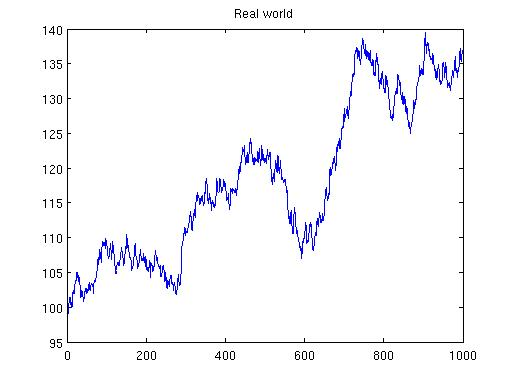
\includegraphics[width=4in]{real1.jpg}
    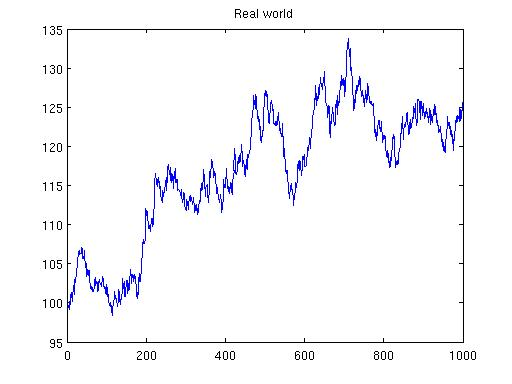
\includegraphics[width=4in]{real2.jpg}
    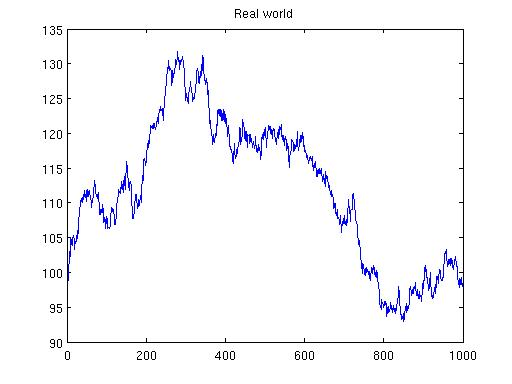
\includegraphics[width=4in]{real3.jpg}
    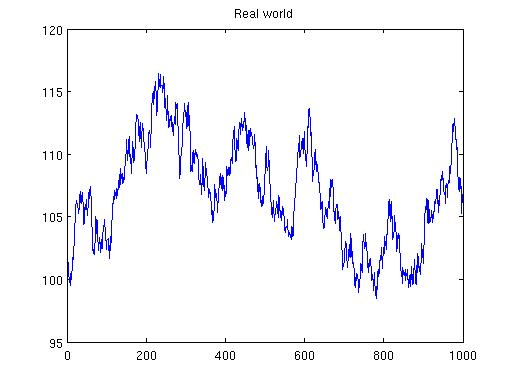
\includegraphics[width=4in]{real4.jpg}
    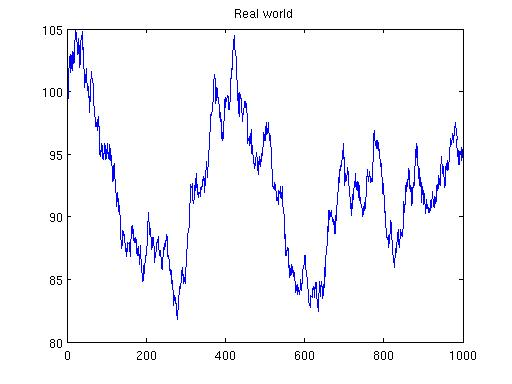
\includegraphics[width=4in]{real5.jpg}
    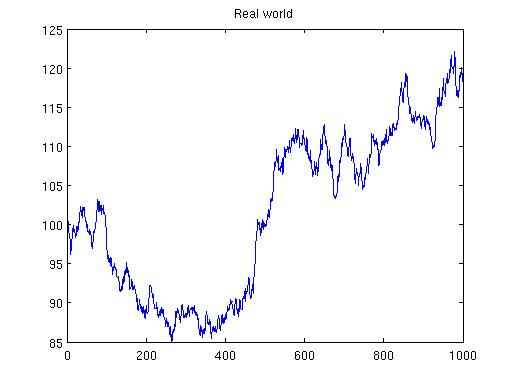
\includegraphics[width=4in]{real6.jpg}
    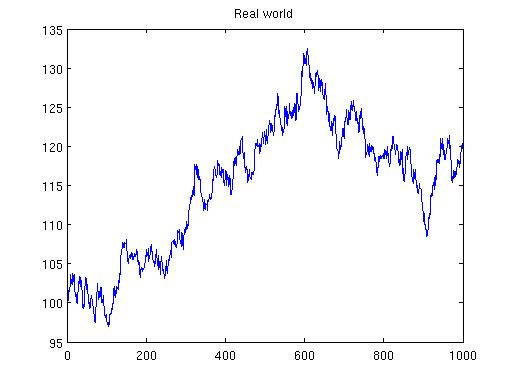
\includegraphics[width=4in]{real7.jpg}
    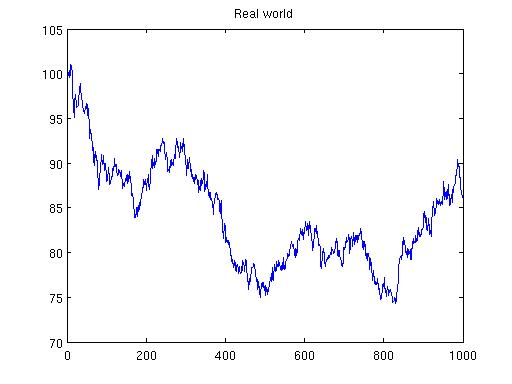
\includegraphics[width=4in]{real8.jpg}
    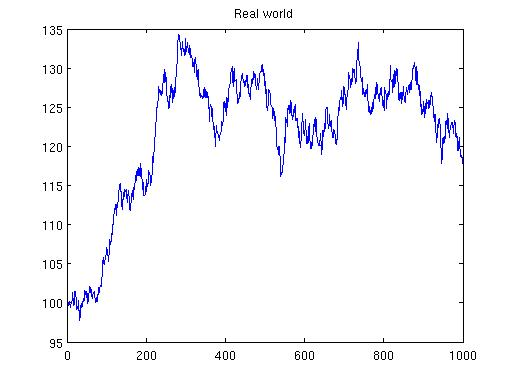
\includegraphics[width=4in]{real9.jpg}
    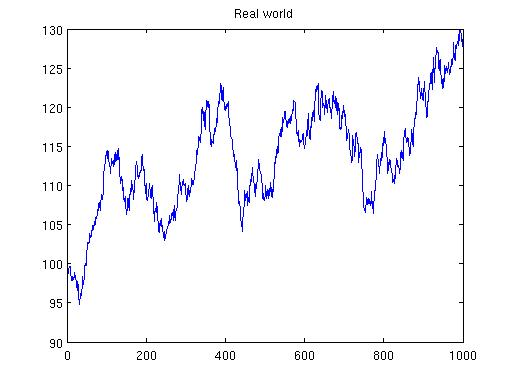
\includegraphics[width=4in]{real10.jpg}
  \end{center}

  \subsection{Risk neutral world}
  \begin{center}
    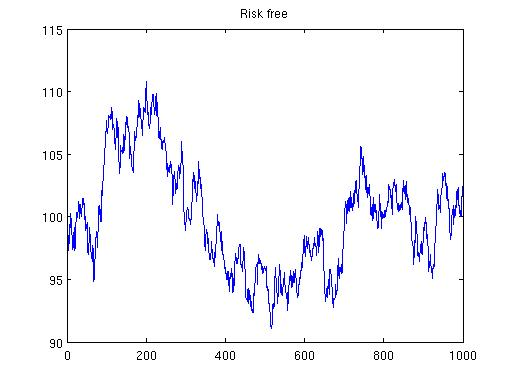
\includegraphics[width=4in]{riskfree1.jpg}
    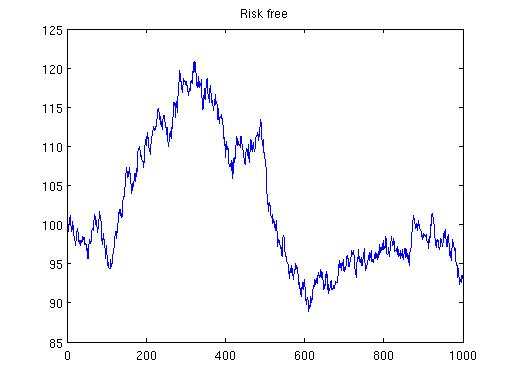
\includegraphics[width=4in]{riskfree2.jpg}
    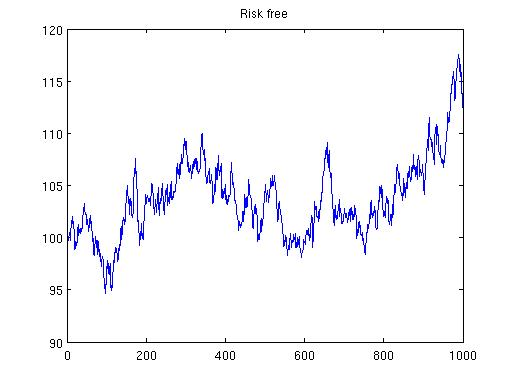
\includegraphics[width=4in]{riskfree3.jpg}
    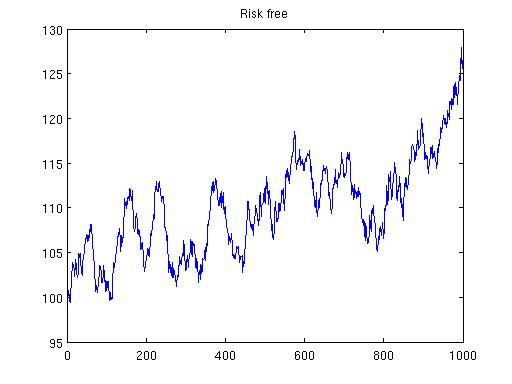
\includegraphics[width=4in]{riskfree4.jpg}
    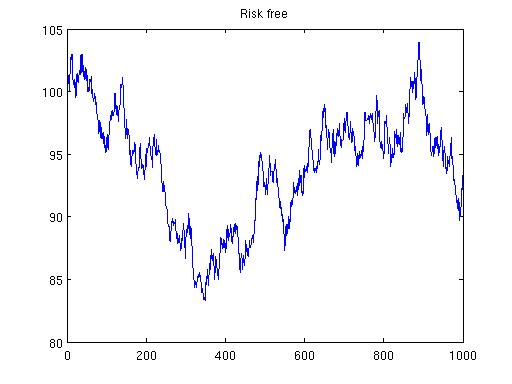
\includegraphics[width=4in]{riskfree5.jpg}
    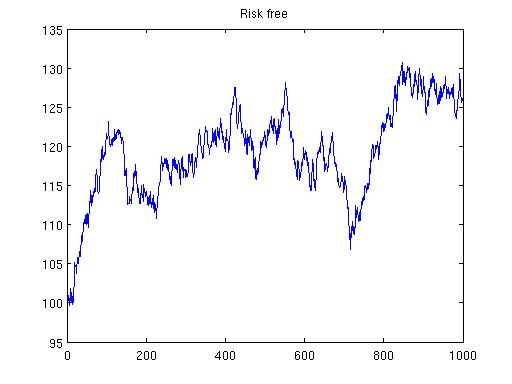
\includegraphics[width=4in]{riskfree6.jpg}
    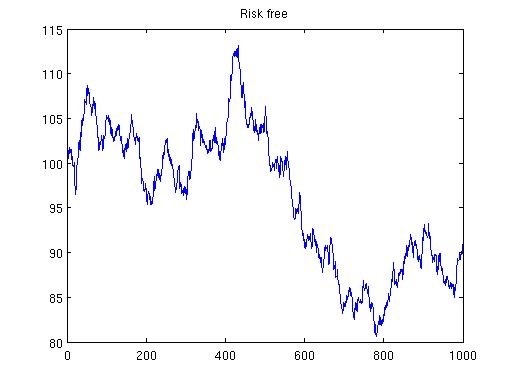
\includegraphics[width=4in]{riskfree7.jpg}
    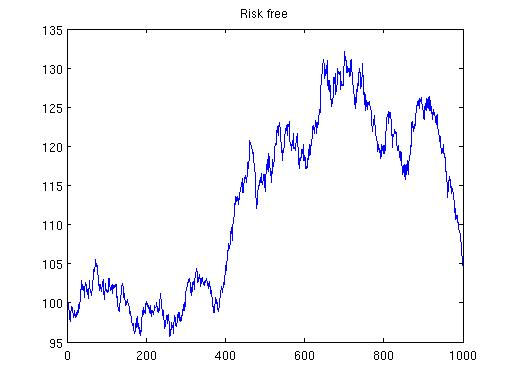
\includegraphics[width=4in]{riskfree8.jpg}
    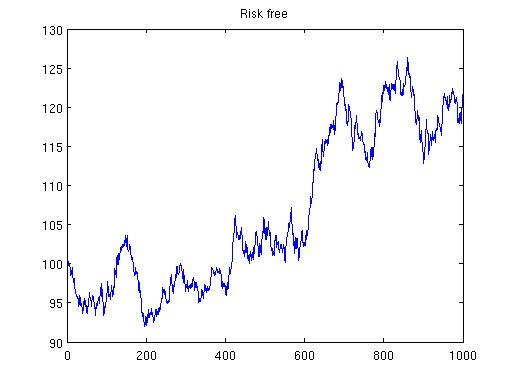
\includegraphics[width=4in]{riskfree9.jpg}
    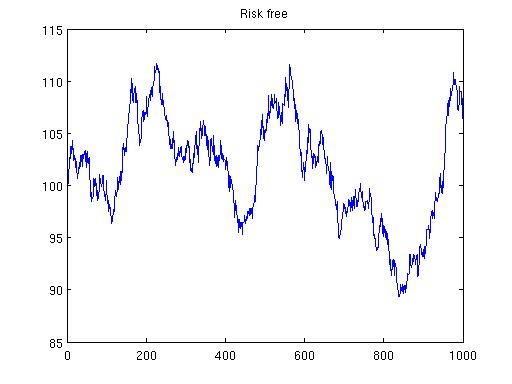
\includegraphics[width=4in]{riskfree10.jpg}
  \end{center}

\newpage
\section{Asian option prices}
  \subsection*{Strike = 105}
    Call = 3.3637\\Put = 5.9741
  \subsection*{Strike = 110}
    Call = 1.9017\\Put = 9.1457
  \subsection*{Strike = 90}
    Call = 12.4386\\Put = 0.34147


\section{Code}
  \subsection{Function to simulate asset price using GBM}
    \lstinputlisting{geometricbrownian.m}
  \subsection{Driver program}
    \lstinputlisting{lab10.m}
\end{document}
